\chapter{FACT}
\begin{wrapfigure}[23]{R}[0pt]{0.45\textwidth}
  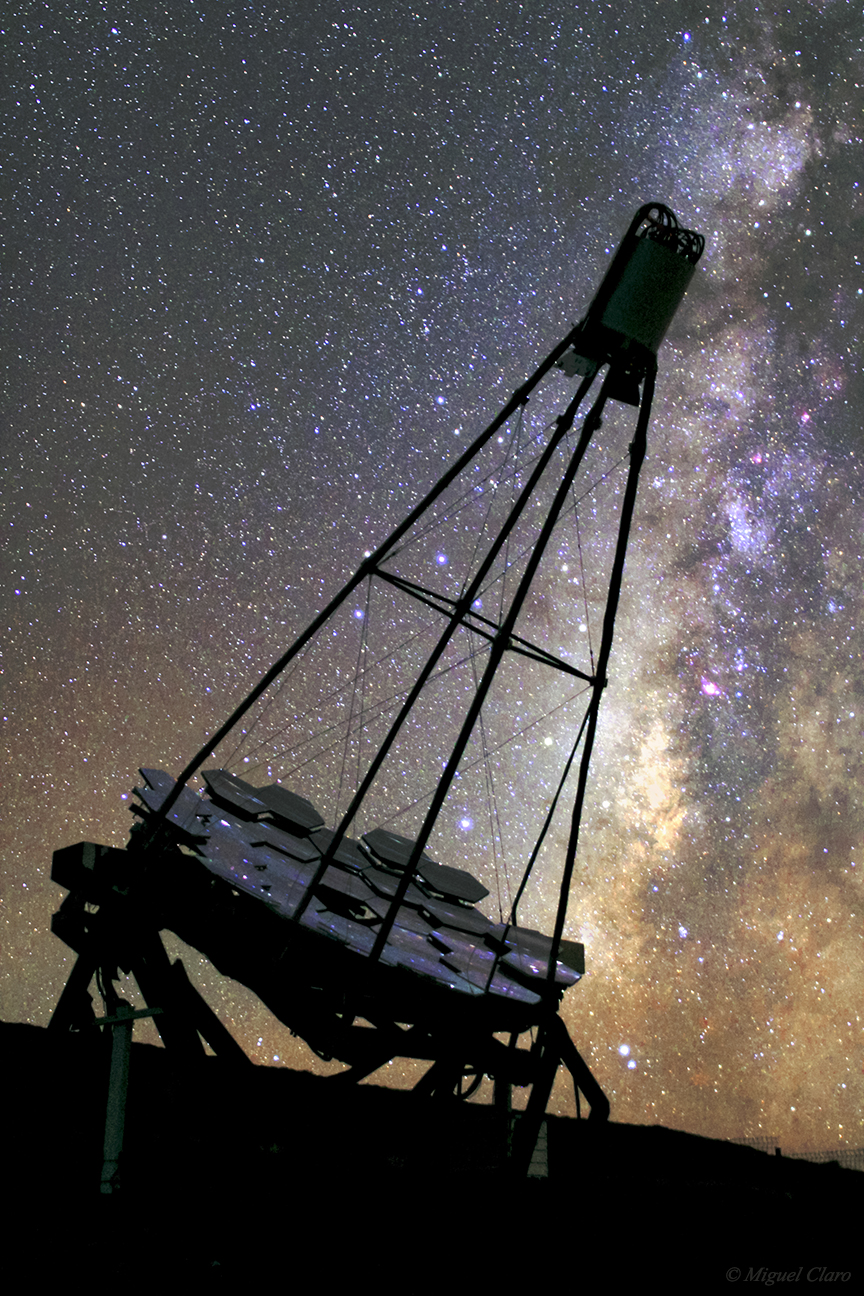
\includegraphics[width=0.45\textwidth]{./images/FACT.jpg}
  \caption{FACT in Observatiosposition \cite{factpic}}
  \label{fig:observ}
\end{wrapfigure}
FACT (First G-APD Cherenkov Telescope) dient der Überwachung von $\gamma$-Quellen, um bei erhöhter Aktivität für genauere Observationen größere Telekope zu informieren. 
Desweiteren erprobt das Telekop die Nutzung von Silizium Photomultipliern (SiMPs), mit welchen es möglich ist auch in Nächten mit starker diffuser Hintergrundstrahlung Quellen zu observieren. 

%Auf einer Höhe von 2200 Meter über dem Meeresspiegel befindet sich das Cherenkov Teleskop auf der kanarischen Insel La Palma. 
FACT befindet sich auf der kanarischen Insel La Palma auf einer Höhe von 2200 Meter über dem Meeresspiegel.
Das Projekt entstand als ein Nachfolgerexperiment des HEGRA CT3 Teleskop, wobei dessen Konponenten aufbereitet und wiederverwertet werden.

Die 30 hexagonalen Spiegel bilden eine Gesamtspiegelfläche von \SI{9.51}{\meter\squared} bei einem Blickfeld von \SI{4.5}{\degree}. 
Die Spiegel sind seit der Neuausrichtung im Davies-Cotton Design ausgerichtet \cite{design-detec}.
Dabei bilden die einzelnen Spiegel eine sphärisch ähnliche Fläche, deren Brennpunkt in die Kamera gelegt ist.

Als erstes Teleskop verwendet FACT SiPMs anstelle von herkömmlichen Photomultiplier Tubes (PMTs). 
Halbleiterdetektoren lassen sich mit einer geringeren Operationsspannung (< \SI{100}{\volt}) betreiben und sind preiswerter als Photomultiplier, was sowohl die Gestaltung des Kameradesigns, als auch die Finanzierung vereinfacht. 
SiPMs sind aufgrund ihrer hohen Sensitivität dazu in der Lage einzelne Photonen zu detektieren und somit auch bei Vollmond noch verwertbare Ergebnisse zu produzieren.
Die Kamera besteht aus 1440 Kamerapixeln, welche jeweils aus einem quadratischen Sensor und einem Plexiglasleiter bestehen. Die einzelnen Oberflächen der hexagonal zulaufenden Plexiglasleiter bilden dabei das Kamerabild.

\chapter{Entstehung von Cherenkov Schauern}
Trifft ein hochenergetisches Teilchen auf die Atmosphäre, löst dieses ein Schauer von Sekundärteilchen aus. Die Energie der erzeugten Sekundärteilchen ist stets geringer als die der einfallende Primärteilchen. Dabei wird zwischen zwei verschiedenen Arten von Schauern unterschieden. 

\textbf{Møglicher weise Tikz picture}

Trifft ein hochenergetisches $\gamma$-Quant auf die Atmosphäre, so wird es wahrscheinlich im Coulombwall der Moleküle durch Paarerzeugung ein Elektronen-Positron-Paar erzeugen. 
Anschließend kann bei hinreichend großer Energie das Elektron durch Bremsstrahlung weitere Photonen erzeugen. 
\begin{eqnarray}
  \gamma \rightarrow& e^{+} + e^{-} \\
  e^{+} \rightarrow& e^{+'} + \gamma \\
  e^{-} \rightarrow& e^{-'} + \gamma 
\end{eqnarray}
Dieser Prozess ist solange fortlaufend bis die Energie der Teilchen zu klein ist, um ein neues Teilchenpaar zu erzeugen. 
Trifft ein geladenes kosmisches Teilchen in die Atmosphäre, so kann dieses über die starke Wechselwirkung, anders als beim elektromagnetischen Schauer, unterschiedliche Sekundärteilchen bilden. 
Dabei entstehen unter anderem neue Hadronen, Mesonen und Myonen, welche wiederum zerstrahlen. 
\begin{eqnarray}
  \pi^{0} \rightarrow& \gamma + \gamma \\
  \pi^{+} \rightarrow& \mu^{+} + \nu_{\mu} \\
  \pi^{-} \rightarrow& \mu^{-} + \bar{\nu}_{\mu}
\end{eqnarray}
Entseht bei der Paarbildung schon früh ein $\pi^{0}$~Meson, so ist der Teilchenschauer kaum von dem eines $\gamma$-Quants zu unterscheiden. 

Bewegt sich ein Teilchen schneller als die Lichtgeschwindigkeit in dem Medium $c_\text{med}$ polarisiert es dieses kurzzeitig. 
Dabei wird eine kohärente Schockwelle in Bewegungsrichtung abgestrahlt. 
Diese bildet einen Mach-Kegel aus, dessen Öffungswinkel $\theta$ von dem Brechungsindex $n$ des Mediums und der Phasengeschwindigkeit der Welle $\beta = v / c_\text{med}$ abhängt.
\begin{equation}
  \cos  \theta = \frac{1}{\text{n} \beta}
\end{equation}
Wird in einem Cherenkov-Teleskop die Größe des Lichtkegels gemessen, bietet dies eine Möglichkeit, die Energie der Primärteilchen zu schätzen. 
\chapter{Observation}
\section{Bildgebende Parameter}
\begin{figure}[H]
  \centering
  \includegraphics[width=0.5\textwidth]{tikz/camera/camera.pdf}
  \caption{Hillas Parameter, anhand derer verschiedene Modelle zur Auswertung des Kamerabildes trainiert werden.}
\end{figure}
Fällt ein Schauer in das Teleskop, erzeugt dieser in der Kamera ein Bild. 
Nachdem Artefakte und äußere Einflüsse bereinigt worden sind, werden anhand der Pixel, die auf den Cherenkovschauer zurückzuführen sind, die Hillas Parameter berechnet. 
Dazu wird eine Gaußverteilung durch die Helligkeit der Pixel gefittet. 
Zu den Hillasparameter zählen:
\begin{itemize}
  \item \textbf{width/length:} Hauptachsen der Ellipse
  \item \textbf{size:} Anzahl an Pixel im Schauer
  \item \textbf{CoG:} Schwerpunkt des Schauers
  \item \textbf{Core of image:} Helligkeit der einzelnen Pixel
  \item \textbf{DISP:} Abstand zwischen Schwerpunkt des Schauers und der gemessenen Quellposition. Anhand der Parameter width und length wird DISP abgeschätzt, um die gemessene Quellposition zu ermitteln. Dabei gibt es zwei mögliche Vorzeichen, welche man durch die Observation der zeitlichen Konzentration der einzelenen Pixel im Schauer abzuschätzen versucht.
  \item \textbf{Source Position:} erwartete Quellposition
  \item \textbf{$\theta$:} Winkel zwischen der gemessenen und echten Quellposition
\end{itemize}
\section{Wobble Observation Strategie}
\begin{wrapfigure}[18]{L}[0pt]{0.53\textwidth}
  \includegraphics[width=0.5\textwidth]{images/wobble.pdf}
  \caption{Wobble observation muss noch zitiert werden. Theme dissertaion}
\end{wrapfigure}
Zur Abschätzung der Untergrundstrahlung in der Wuellregion (On-Positio) werden stellen am Himmel beobachtet, an denen keine Quellen zu erwaten (Off-Position) sind.
Die gemessenen Untergrundraten können dann von den Messungen in der Quellregion subtrahiert werden um die \textbf{tatsächliche} Signalrate \textbf{zu bestimmen/ abzuschätzen}.
%Zur Bestimmung des Aktivität einer Quelle, werden bei deren Observation einerseits Daten aus der Quellregion (On-Position), sowie Daten aus ähnlichen Richtungen einer Position bei denen nur diffuse Hintergrundstrahlung (Off-Position) erwatet wird genommen. Aus der Beziehung der On- und Off-Daten wird versucht die statistische Effekte der Hintergrundstrahlung bei der Quellobservation zu minimieren.

Die Wobble Observation Strategie zeichnet aus, dass im Gegensatz zur klassischen Methode, nicht hintereinander On/Off Postionen beobachtet werden. 
Stattdessen wird die erwartete Quellpostion \SI{0.6}{\degree} neben die Kameraachse gelegt. 
Dies hat zur Folge, dass es mehrere Positionen mit dem selben Abstand und Symmetrie zur Kameraachse gibt. 
Bei der Standardanalyse von Fact können so neben der On-Position, fünf Off-Positionen mit demselben Winkel zur Kameraachse gemessen werden. 
Somit ergibt sich für jedes Datensample jeweils ein $\theta_\text{on}$ und fünf $\theta_\text{off}$. 
Für sehr kleine $\theta$ Winkel kann oftmals geschlossen werden, dass das gemessene Teilchen aus der Richtung der Quelle kam und vermutlich ein $\gamma$-Quant ist. 
Da der Hadronuntergrund isotrop in alle Richtungen verteilt auftritt, sollte bei hadronischen Schauern $\theta^{2}$ in etwa gleichverteilt seien. 
Zu den Vorteilen dieser Methode zählt, dass keine extra OFF-Daten genommen werden müssen. 
Somit ist es möglich, die Messzeit zu maximieren. 
Desweiteren kann durch die gleichzeitige Datennahme davon ausgegangen werden, dass für die On/Off-Positionen annähernd die selben Wetterbedingungen gelten. 

\chapter{Überwachtes Maschinelles Lernen}
Zur Auswertung der Datenmenge von 300 GB bis 1 TB \cite{MaxNoethe}, die FACT jede Nacht aufnimmt, werden maschinelle Lernmethodenen verwendet. 
Maschinelles Lernen kann dazu genutzt werden, Muster und Strukturen auf Datensätzen zu erkennen und zukünftige Ereignisse hervorzusagen. 
Dabei wird zwischen überwachtem und unüberwachtem Lernen unterschieden.

Unüberwachtes Lernen zeichnet sich dadurch aus, dass versucht wird, auf dem Trainingsdatensatz Muster zu erkennen.  

Ziel des überwachten Lernens ist es, bei einem gegebenen Trainingsset, welches aus Eingangsvariablen $X$ und Zielvariablen $y$ besteht, Modelle zu finden, welche $X$ bestmöglich auf $y$ abbilden. 
Zunächst muss dafür das Modell trainiert werden. 
Dafür wird ein Datensatz, bei dem die Zielvariablen $y$ bekannt sind, in zwei Teile aufgeteilt, dem Trainings- und dem Testdatensatz. 
Dabei wird das Modell auf den Trainingsdatensatz optimiert und anschließend auf dem Testdatensatz evaluiert. 
Hier ist darauf zu achten, dass das Modell nicht nur den Trainingsdatensatz auswendig lernt (Übertraining), sondern allgemein genug bleibt auch ähnliche Datensätze genau vorherzusagen. 
Dies geschieht durch Beschränkung der Modelle. 
Durch Berechnung von Evaluationsmetriken auf dem Testdatensatz, welcher unabhänging von dem Trainingsdatensatz ist, kann geprüft werden, ob das Modell allgemein genug ist oder an Übertraining leidet.
\section{Entscheidungsbaum}
\begin{wrapfigure}[12]{R}[0pt]{0.5\textwidth}
  \centering
  \includegraphics[width=0.5\textwidth]{./tikz/tree/tree.pdf}
  \caption{Entscheidungsbaum der Tiefe 2 bei Gamma Handron Seperation}
\end{wrapfigure}
Ein Entscheidungsbaum beginnt mit einem Wurzelknoten. Ausgehend von diesem wird durch Abfrage von verschiedenen Bedingungen eine Auswahl an Folgeknoten getroffen. 
In der Regel werden in der Datenanalyse binäre Entscheidungsbäume genutzt, \textbf{aufgrund dessen das sich jede komplexere Abfrage auf eine Verknüpfung mehrer binären Abfragen reduziere lässt.}
% aufgrund dessen das sich jedes komplexeres auf ein binäres reduzieren lässt.
Entsprechend eines Schwellwertes wird der Datensatz aufgeteilt, sodass die entstehenden Untergruppen möglichst homogen werden. 
%sodass der Baum entsprechend an einem threshold wert die Daten an jedem Knoten in die zwei folgenden Knoten aufspaltet. 
%Dieser Prozess wird solange durchgeführt bis ein Blatt erreicht wird, in dem sich ausschließlich Ereignisse einer Klasse befinden und eine erneute Aufspaltung keinen Erkenntnissgewinn bringt. 
\textbf{Dieser Prozess wird solange durchgeführt bis nach einer Abfrage alle Ereignisse ausschließlich einer Klasse angehören oder eine erneute Aufspaltung keinen Erkenntnissgewinn bringt. Die Enden einer solchen Abfrage werden als Blätter bezeichnet und geben die Vorhersage des Baums an.}
Die Anzahl an Knoten die durchlaufen werden bis das letzte Blatt errreicht ist, wird als Tiefe der Bäume bezeichnet.
Der Baum kann entsprechend verschiedener Kriterien gebaut werden.
Zu den gängigen gehört die Entropie oder der Gini-Index \cite{MAchineLearningBook}. 
Zu den Vorteilen eines Entscheidungsbaums zählt, dass dieser gut interpretierbar und nachvollziehbar ist. 
Allerdings kommt es ohne Beschränkung schnell zum Übertraining.
\section{Random Forest}
Ein Random Forest besteht aus vielen unabhängigen Entscheidungsbäumen.
Jeder Entscheidungsbaum zieht bei der Erstellung immer nur eine Teilmenge aus allen Attributen.
Zur Klassifizierung wird anschließend eine Mehrheitsabstimmung über alle Entscheidungsbäumen durchgeführt.
Dadurch, dass die einzelnen Bäume unterschiedlich aufgebaut sind und über die einzelnen Lerner gemittelt wird, ergibt sich ein Modell mit reduzierter Varianz im Gegensatz zum Entscheidungsbaum, welches robuster gegen Übertraining ist.
\section{Extra Boosted Decisiontrees}
Hier kommt später Inhalt hin
\section{Evaluationsmetriken}
Zum Testen inwiefern sich die Modelle auf den Datensätze verhalten werden zweierlei Metriken zu der Beurteilung der Klassifizierer benutzt.
\subsection*{Receiver Operating Characteristic}
\begin{wrapfigure}[12]{R}[0pt]{0.4\textwidth}
  \centering
  \includegraphics[width=0.4\textwidth]{./Plots/roc_info.pdf}
  \caption{ROC Score zweier verschiedenen Modelle}
  \label{fig:roc}
\end{wrapfigure}
Zum Vergleich von verschiedenen binären Klassifizern ist die ``Receiver Operating Characteristic Curve'' ein Maß für die Güte der Seperation. 
Dafür wird zunächst der Konfidenzwert des Klassifizierer berechnet. 
Dies ist ein Wert zwischen den Werten 0 und 1, welcher die Sicherheit wiederspiegelt, dass die Vorhersage den Zielklassen 0 oder 1 entspricht.
Für alle möglichen Konfidenzwerte wird der prozentuale Anteil an richtig klassifizierten Ereignissen der Klasse 1 (TPR) und an Falschklassifizierten der Klasse 0 (FPR) berechnet. 
Bei der ROC Curve wird die TPR gegen die FPR Rate aufgetragen. 
Ein Beispiel ist in Abbildung \ref{fig:roc} zu sehen.
Für einen guten Klassifizier strebt die Kurve bei kleinen FPR gegen hohe TPR. 
Angeonommen der Klassifier ist nicht in der Lage zwischen den beiden Klassen zu separieren, dann steigen die TPR und FPR gleichermaßen. 
Anhand der Fläche unter der Kurve können die Güten anhand von Zahlen verglichen werden.
\subsection*{Li und Ma Signifikanz (nochmal komplett bearbeiten)}
% Muss noch verbessert werden.
Aufgrund der Begrenztheit der Dektorsensitivität muss bei der Analyse von möglichen Quellen sorgsam mit den Daten zur Bestimmung der Sicherheit einer Quelle umgegangen werden.
Dabei kann nicht das Signal einer Quelle isoliert gemessen werden. 
Stattdessen muss eine Sicherheit auf das Signals welches aus Richtung der Quelle $N_\text{on}$ und des Hintergrunds $N_\text{off}$ gegeben werden, dass das gemessene Signal nicht nur statistisches Rauschen ist.
% //////////////////////////////
Ein möglicher Anatz ist die Li and Ma Signifikanz \cite{liandma}, bei der über einen statistischen Hypothesen Test geprüft wird ob das Signal $N_\text{S}$ nur ein Teil des Untergrunds $N_\text{B}$ ist. 
Aus dem Verhältniss der Messzeiten der On- und Off-Position $\alpha$ wird die Hintergrundstrahlung berechnet. 
Aus der Differenz der On-Region und der Hintergrundrate lässt sich so die Signalrate bestimmen. 
Durch das Aufstellen der Maximum Liklihood Funktion und des anschließenden Test ergibt sich für die Li and Ma Signifikanz
\begin{equation}
S = \sqrt{2} \left( N_\text{on} \ln \left[ \frac{1+ \alpha}{\alpha}\left( \frac{N_\text{on}}{N_\text{on} + N_\text{off}} \right) \right] + N_\text{off} \ln \left[ \left( 1+ \alpha \right) \left( \frac{N_\text{off}}{N_\text{on} + N_\text{off}} \right) \right] \right)^{1/2}.
\end{equation}

\chapter{Quellen}
In dieser Arbeit werden Datensätze von zwei verschiedenen Quellen verwendet. 
Beide dieser Quellen scheinen bereits gut verstanden und können zum Vergleich zu anderen Arbeiten verwendet werden.
\section{Krebs Nebel}
In einer Entfernung von 6400 Lichtjahren befindet sich im Sternzeichen Stier der Überrest der ersten und letzten dokumentierten Supernovaexplosion, die auf das Jahr 1054 datiert ist. 
Die Überreste erstrecken sich über eine Fläche von 6 Bogenminuten Länge und 4 Bogenminuten Breite. 
In der Mitte des Krebs Nebels liegt ein Neutronenstern.
Aufgrund seines konstanten Strahlungsflusses ist der Krebsnebel eine Standard- und Kalibrierungsquelle in der Gammaastronomie.
Er gilt dabei als stärkste Quelle am Himmel. 
Viele wissentschaftliche Arbeiten nehmen diesen als Referenzwert, um ihre Messwerte zu vergleichen. 

\section{Markarian 501}
Im Sternbild Herkules befindet sich in einer Entfernung von in etwa 500 Lichtfahren der Blazar Markarjan. 
In dessen Zentrum befindet sich ein \num{0.9} bis \num{3.4} Milliarden Sonnenmassen schweres schwarzes Loch, dessen Jet in Richtung Erde gerichtet ist.
Auch dieser gilt als einer der stärksten Gammastrahlungsquellen.
